\section{Reference architecture for IaaS clouds}
\label{sec:moreno}


% if this architecture is based on abstracted concepts and is not tied coupled
% to specific technology, it is inspired by existing IaaS managers. Thus the
% question of how it scales with massively distributed clouds is relevant.

% \item Current IaaS managers almost same entities: virtual machines, storage,
% image, network, security. That explains why they have implemented similar 
% services \cite{peng:2009}.

% \item Moreno et al. have proposed a reference architecture that covers 
% services that manipulate such entities \cite{moreno2012iaas}.

% \item Figure \ref{fig:moreno} depicts this reference architecture. Even
% if this architecture is based on abstracted concepts and is not tied coupled
% to specific technology, it is inspired by existing IaaS managers. Thus the
% question of how it scales with massively distributed clouds is relevant.

% \item In the following paragraphs we detail for services concerned 
% challenges that need to be solved to scale with massively distributed 
% clouds. For the construction	

Infrastructure as a service (IaaS) is a model where companies consume computing
resources produced by external cloud providers. This model has lead to a 
structure similar to the electricity market: in the same way electrical 
providers have build huge infrastructures for generating and transporting 
energy, cloud providers now leverage data-centers that can host more than tens 
of thousands of servers.

As this market is dominated by few actors (Amazon, Rackspace, ...), de facto
standards have emerged. Recent studies like \cite{peng:2009} have compared state
of the art open-source IaaS manager: it appears that they almost manipulate same
entities like virtual machines, disk images and storage services. Despite 
efforts made on cloud interoperability, standardization efforts seem still
unsuccessful as there does not exist a widely accepted standard.

Moreno et al. have proposed a reference architecture \cite{moreno2012iaas} 
for IaaS clouds, that covers services that are needed for building a Cloud OS. 
Figure \ref{fig:moreno} depicts this proposition: with this model, each aspect 
of the cloud is supervised by a specific manager. Furthermore this model enables
the abstraction of how is implemented the underlying infrastructure. Authors 
argues that following a reference architecture is a key to the widespread 
adoption of IaaS clouds.

However, the proposed architecture does not give any specific hints for
building a massively distributed Cloud OS: indeed the question whether such 
system is scalable or not is relevant. Focusing on managers that are suitable 
for virtual machines provisioning, we detail in following paragraphs the 
challenges that need to be solved to scale with massively distributed clouds:


\begin{description}

	\item [Distributed VM scheduling] \textit{(Virtual machine manager and 
	Scheduler)} : In a massively distributed cloud computing resources are 
	spread all over the network. Thus the processus of finding adequate 
	servers for hosting/relocating VMs can become complex. The Virtual
	machine manager and the resource scheduler should leverage collaboration 
	that scales with the growth of the infrastructure, whether it contains 
	hundreds or millions of servers.

	\item [Image and Storage managers] : Virtual machines are based on disk
	image which can be given by cloud provider (standard images) or uploaded
	by users (customized images). It is possible to persist VM states for
	suspending/resuming VM execution or for fault tolerance purpose. We see two 
	challenges here:

	\begin{itemize}

		\item As every virtual machine will be based on disk image, users
		will be provided a set of default image that can be used. They will
		be free to customize a given image with additional softwares and
		configurations. A user must be able to access its images on every
		nodes composing the Cloud OS, which involves distributed file 
		storage and replication of these customized images.

		\item Being able to store a large amount of virtual machines 
		snapshots: as each replica weights several gigabytes, a massively 
		distributed cloud have to provides storage mechanisms for storing 
		thousands of VM replicas.

	\end{itemize}

	\item [Managing virtual network (Network manager)] : A virtual 
	environment is the aggregation of virtual machines interconnected over
	a virtual network. While interconnection is not a problem in a mono-site
	infrastructure, managing virtual networks that link geographically spread
	virtual machines is tedious task due to IP overlapping and VM 
	relocalization. A Cloud OS that manages massively distributed clouds must 
	provide scalable network mechanisms for interconnecting virtual machines of 
	a same virtual environment spread over several sites.

	\item [Accounting and Auditing] : A Cloud OS must provide mechanisms for
	analyzing users activity and infrastructure usage to improve security and 
	quality of service. As more data processed leads to more accurate analysis, 
	a massively distributed Cloud OS must provide mechanisms that enables the
	collect, the storage and the processing of large operating data. Furthermore
	these mechanisms must be able to work in geographically spread context.

\end{description}


% Recent studies have showed that state of the art IaaS manager \cite{peng:2009}
% were constructed over the same concepts, and some authors have proposed a 
% reference architecture for builing IaaS infrastructure. In \cite{moreno2012iaas}
% authors proposed the concept of Cloud OS: they aimed at providing abstractions 
% for services that compose current IaaS managers. Every single functions of 
% current IaaS manager is detailled. Figure \ref{fig:moreno} depicts this 
% reference architecture.

\begin{figure*}
	\centering
	\vspace*{-1cm}
	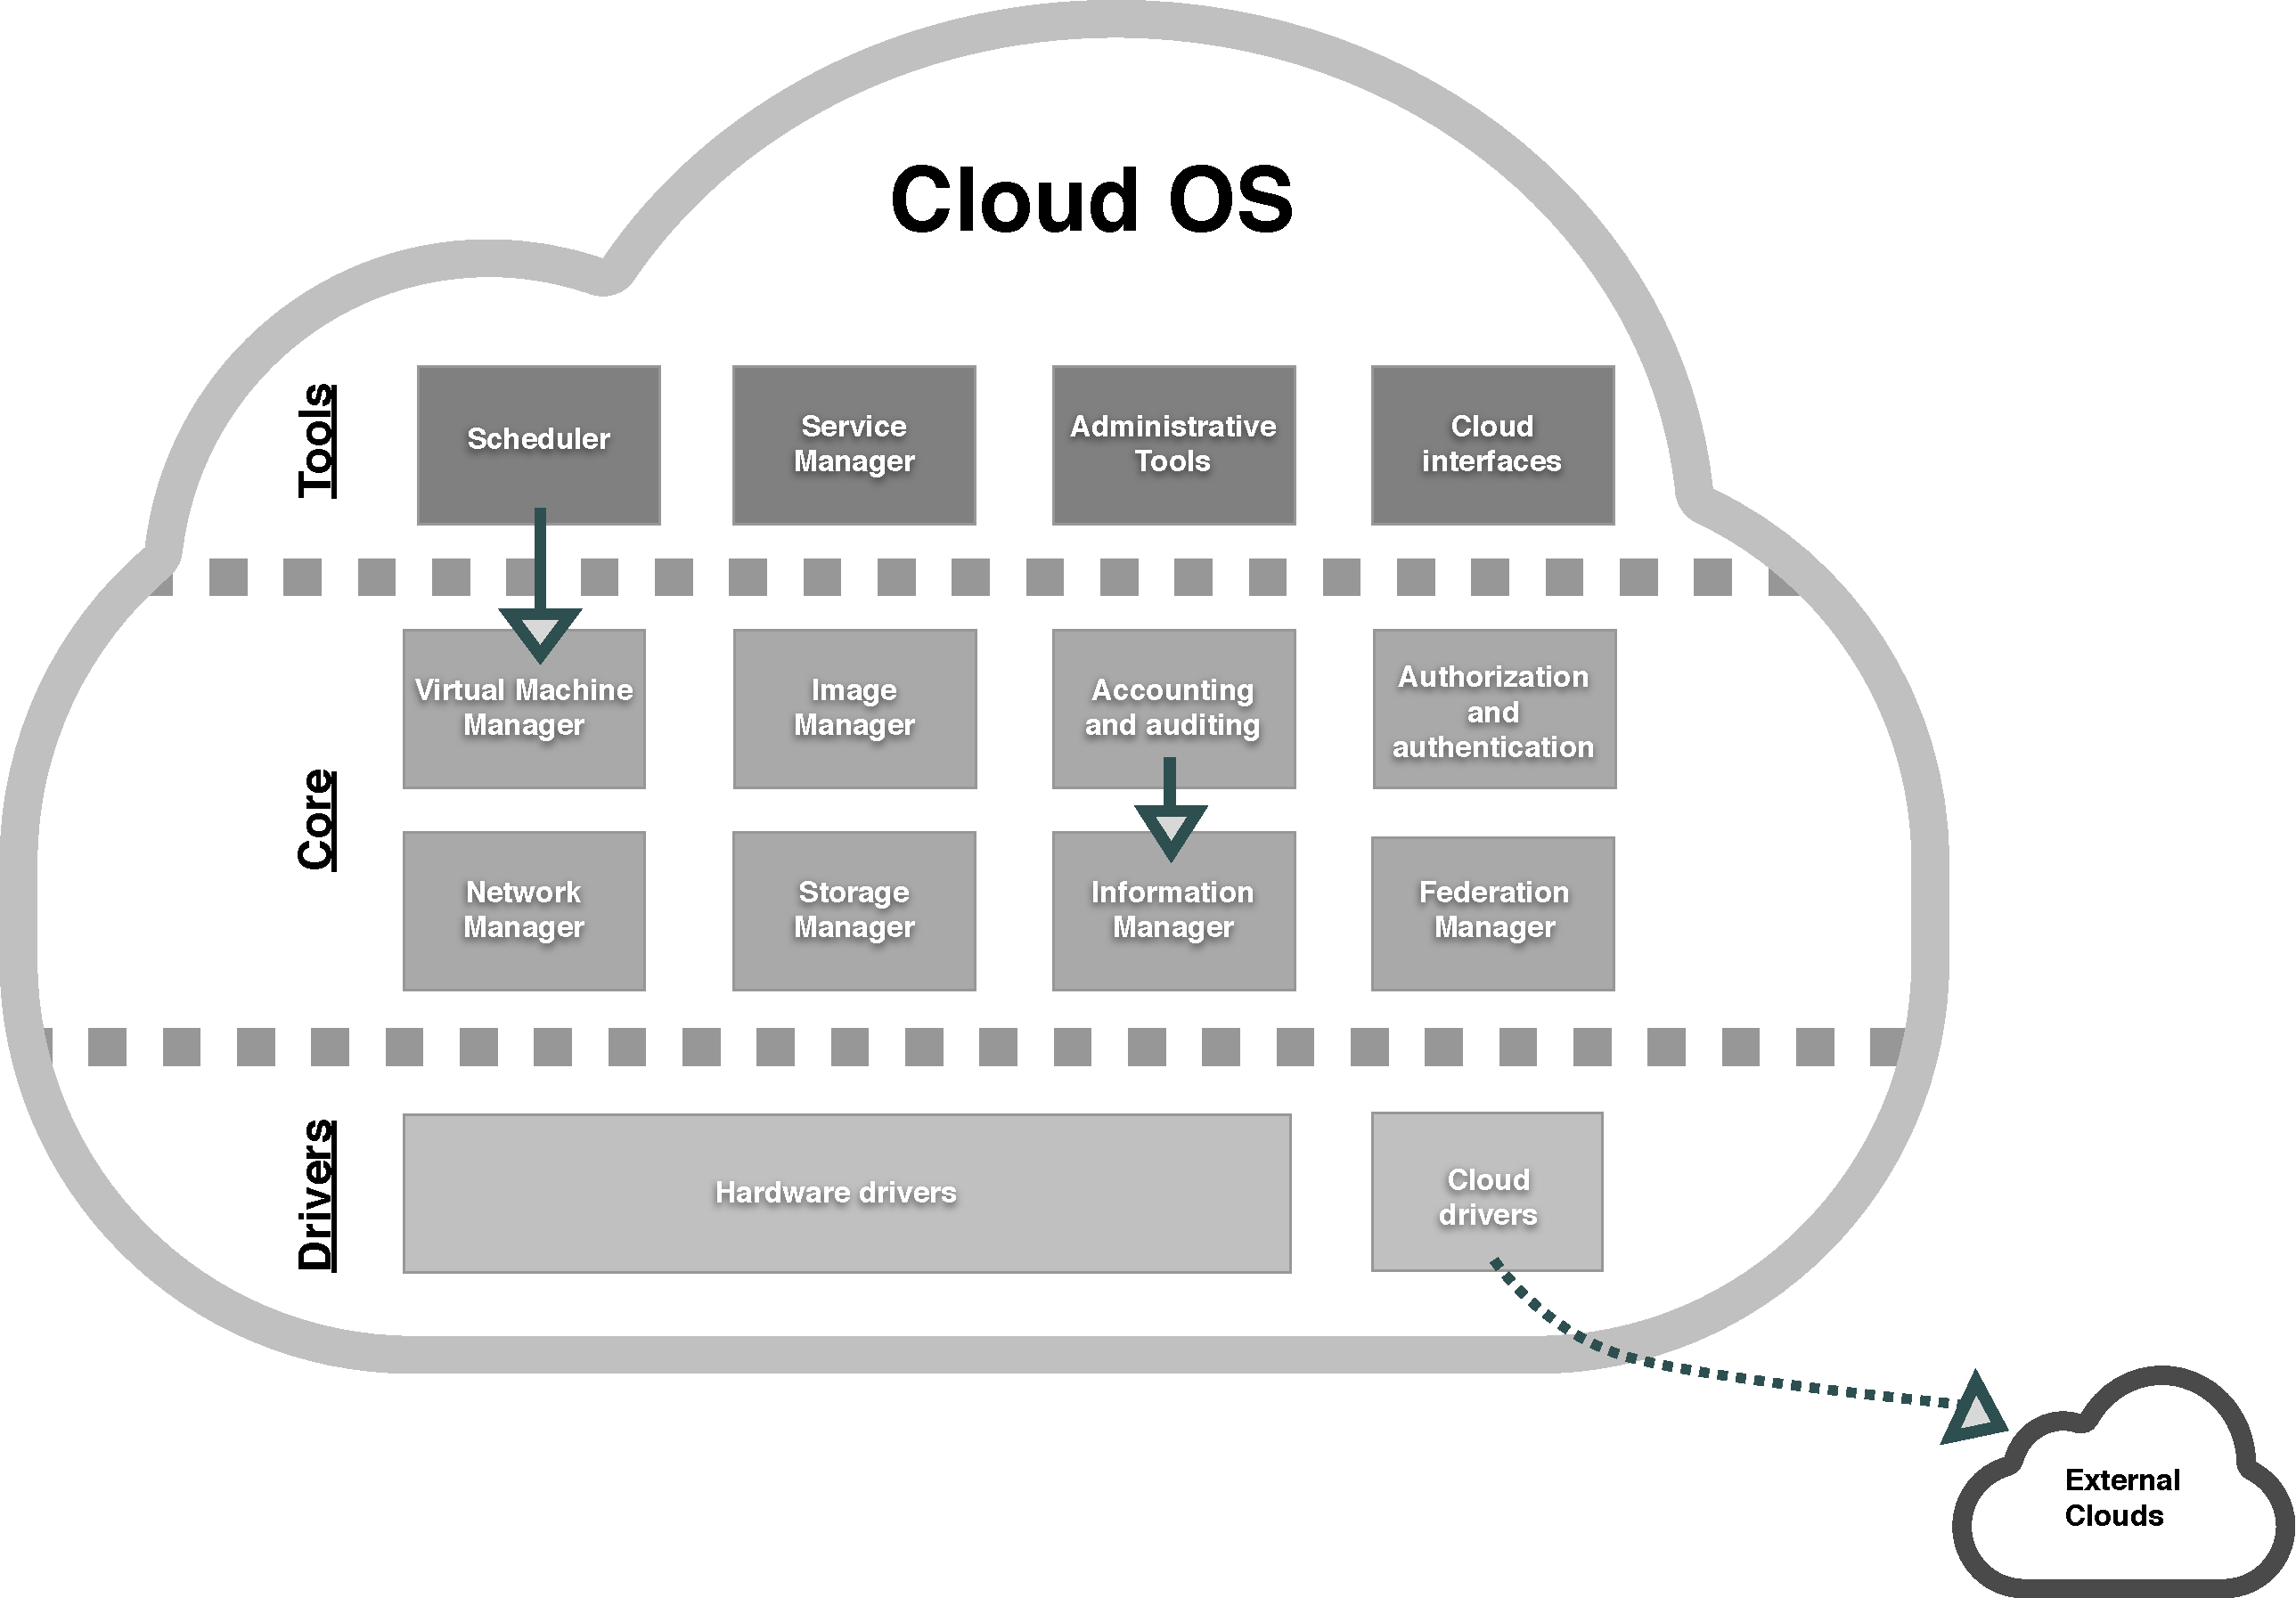
\includegraphics[width=1.1\linewidth]{Figures/moreno.pdf}
	\caption{Architecture proposed by Moreno et al.\cite{moreno2012iaas}.}%
	\label{fig:moreno}%
	% \vspace*{-1cm}
\end{figure*}

As main challenges that need to be solved have been introduced, we propose in 
section \ref{sec:lucos} specifications for a Cloud OS that effectively operate
massively distributed clouds over a geographically spread infrastructure: the 
LUC-OS.

